\documentclass[10pt]{homeworg}

\usepackage{bm}
\title{Homework 1}
\author{Kevin Yang - 50244152}


\begin{document}

\maketitle

\exercise
Let $X = (x_1, x_2, \ldots, \boldsymbol x_n)$ \\
\vspace{0.5cm}
$x_i \sim Pois(\lambda)$  \hspace{2cm} $\lambda \sim \Gamma(\alpha, \beta)$
\\
We have that:
\begin{align*}
P(\lambda \mid X) &= \frac{P(X \mid \lambda)P(\lambda)}{P(X)}\\
				  &\propto P(X \mid \lambda)P(\lambda)\\
				  &\propto \lambda^{n\bar{x}}e^{-n\lambda}\lambda^{\alpha-1}e^{-\beta\lambda}\\
				  &= \lambda^{n\bar{x}+\alpha-1}e^{-(n+\beta)\lambda}
\end{align*}

Therefore, $P(\lambda \mid X) \sim \Gamma(n\bar{x}+\alpha, \beta+n)$ and the Gamma distribution is conjugate to the Poisson distribution.

\exercise
Let $s = (s_1, s_2, \ldots, s_n)$, $s' = (s_1', s_2', \ldots, s_n')$ and $s_{-i} = (s_1, \ldots, s_{i-1}, s_{i+1}, \ldots, s_n)$\\
We will show that Gibbs sampling satisfies the detailed balance equation: $\pi(s)P(s,s')=\pi(s')P(s',s)$\\

w.l.g consider an update for $s_1$\\
\vspace{0.5cm}

\textit{Case 1:} $s_{-1} \neq s_{-1}'$
\begin{align*}
\pi(s)P(s,s') = \pi(s')P(s',s) = 0
\end{align*}


\textit{Case 2:} $s_{-1} = s_{-1}'$
\begin{align*}
\pi(s)P(s,s') &= \pi(s)P(s_1' \mid s_{-1}')\\
			  &= \pi(s)\frac{\pi(s')}{\sum_z \pi(z, s_{-1}')}\\
			  &= \pi(s')\frac{\pi(s)}{\sum_z \pi(z, s_{-1})}\\
			  &= \pi(s')P(s_1 \mid s_{-1})\\
			  &= \pi(s')P(s',s)
\end{align*}

Consider the move from $s$ to $s'$. The acceptance probability for MH will be

\begin{align*}
\frac{\pi(s')P(s',s)}{\pi(s)P(s,s')} = 1
\end{align*}




\exercise
a)
\begin{center}
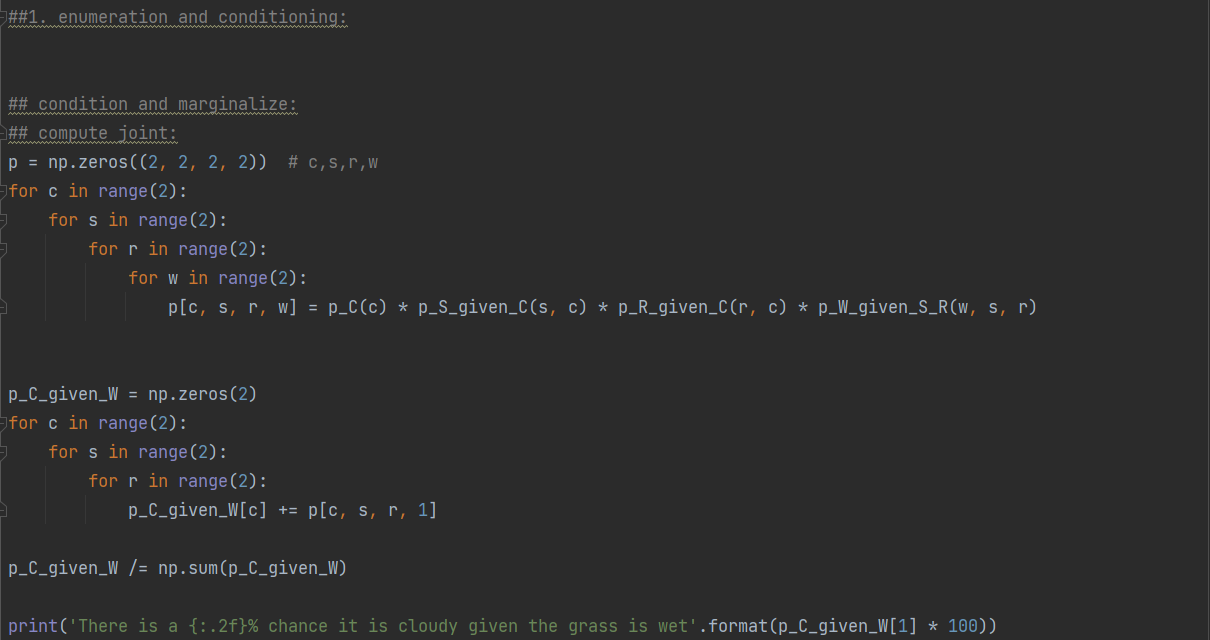
\includegraphics[scale=0.7]{figures/q3_a.PNG}
\end{center}


b)
\begin{center}
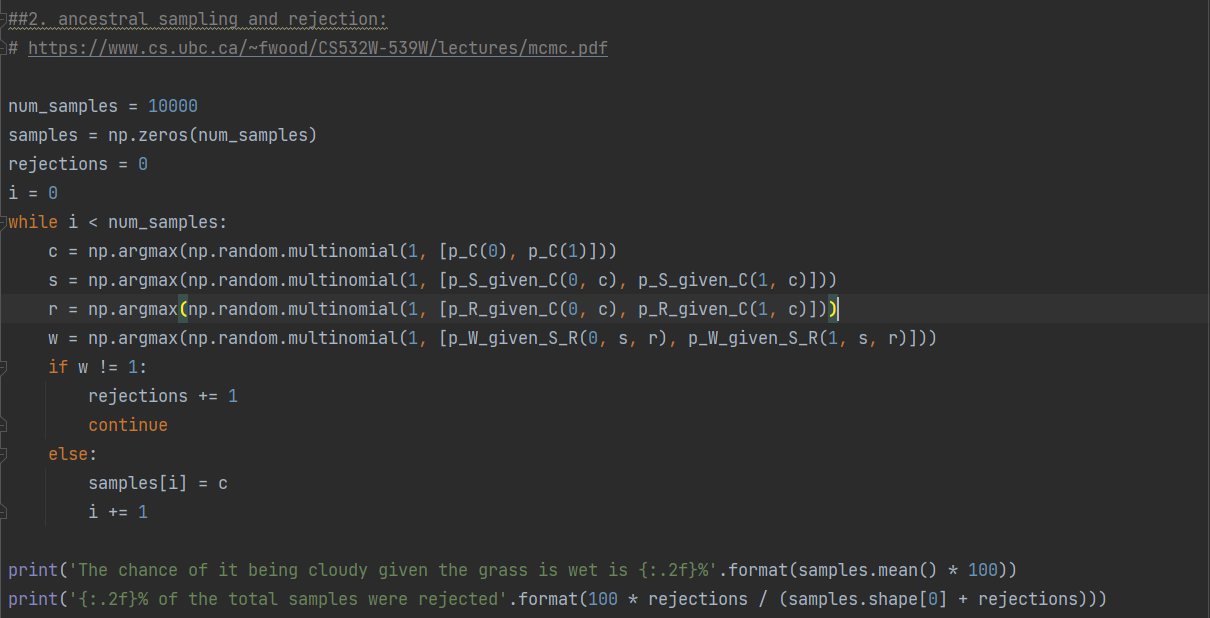
\includegraphics[scale=0.7]{figures/q3_b.PNG}
\end{center}


c)
\begin{center}
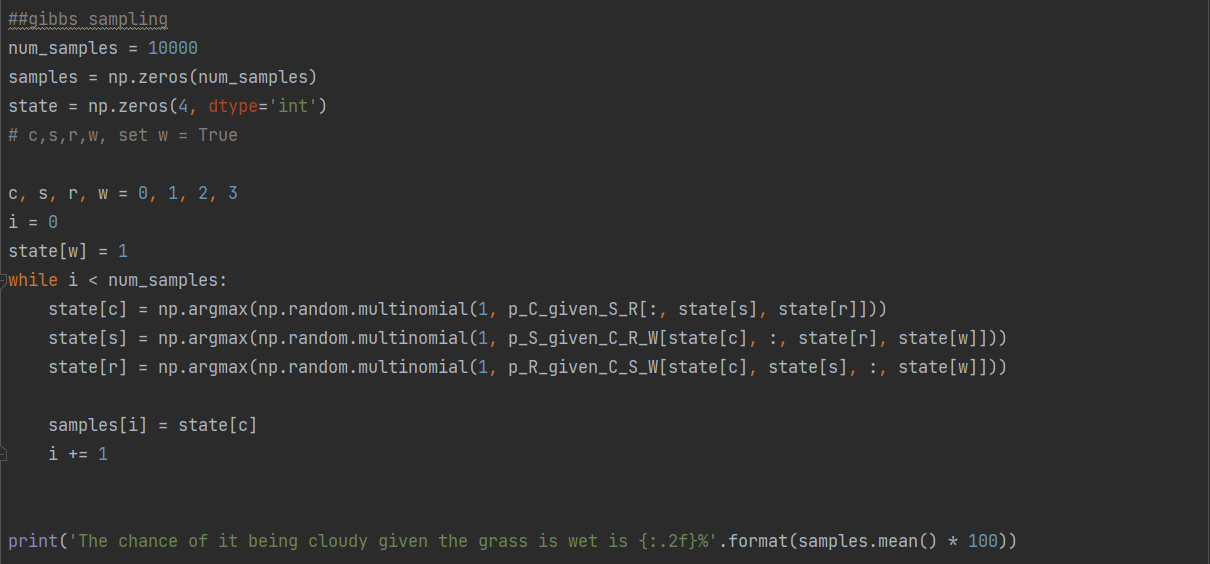
\includegraphics[scale=0.7]{figures/q3_c.PNG}
\end{center}

Results:
\begin{center}
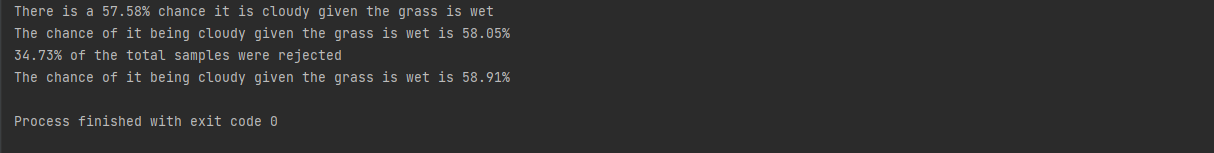
\includegraphics[scale=0.7]{figures/q3_results.PNG}
\end{center}



\exercise 
\textbf{MH within Gibbs on blocks $w$ and $\hat{\boldsymbol t}$}:\\
\\
\underline{$\boldsymbol w$ block}

Let $q(\boldsymbol w,\boldsymbol w')$ be the proposal distribution. We also have that,

\begin{align*}
\pi(\boldsymbol w) &\propto p(\boldsymbol t,\boldsymbol x,\sigma^2,\boldsymbol w,\alpha)\\
	   &= \prod_{n=1}^N \frac{1}{\sigma \sqrt{2\pi}} e^{-\frac{1}{2}(\frac{\boldsymbol t_n-\boldsymbol w^T \boldsymbol x_n}{\sigma})^2} \prod_{d=1}^D \frac{1}{\sqrt{2\pi\alpha}} e^{-\frac{1}{2} (\frac{\boldsymbol w_d}{\sqrt{\alpha}})^2}
\end{align*}

So the update probability is,

\begin{align*}
r &= \frac{\pi(\boldsymbol w')q(\boldsymbol w',\boldsymbol w)}{\pi(\boldsymbol w)q(\boldsymbol w, \boldsymbol w')}\\
\vspace{0.5cm}
  &= \frac{\prod_{n=1}^N \frac{1}{\sigma \sqrt{2\pi}} e^{-\frac{1}{2}(\frac{\boldsymbol t_n-\boldsymbol w'^T\boldsymbol x_n}{\sigma})^2} \prod_{d=1}^D \frac{1}{\sqrt{2\pi\alpha}} e^{-\frac{1}{2} (\frac{\boldsymbol w'_d}{\sqrt{\alpha}})^2} q(\boldsymbol w',\boldsymbol w)}{\prod_{n=1}^N \frac{1}{\sigma \sqrt{2\pi}} e^{-\frac{1}{2}(\frac{\boldsymbol t_n-\boldsymbol w^T\boldsymbol x_n}{\sigma})^2} \prod_{d=1}^D \frac{1}{\sqrt{2\pi\alpha}} e^{-\frac{1}{2} (\frac{\boldsymbol w_d}{\sqrt{\alpha}})^2} q(\boldsymbol w, \boldsymbol w')}\\
  \vspace{0.5cm}
  &\propto  \frac{\prod_{n=1}^N e^{-\frac{1}{2}(\frac{\boldsymbol t_n-\boldsymbol w'^T\boldsymbol x_n}{\sigma})^2} e^{-\frac{1}{2}(\boldsymbol w'^T(\alpha I)^{-1}\boldsymbol w')} q(\boldsymbol w',\boldsymbol w)}{\prod_{n=1}^N e^{-\frac{1}{2}(\frac{\boldsymbol t_n-\boldsymbol w^T\boldsymbol x_n}{\sigma})^2} e^{-\frac{1}{2}(\boldsymbol w^T(\alpha I)^{-1}\boldsymbol w)} q(\boldsymbol w, \boldsymbol w')}\\
  &= \frac{e^{-\frac{1}{2}(\boldsymbol t - \boldsymbol x\boldsymbol w')^T(\sigma^2 I)^{-1}(\boldsymbol t-\boldsymbol x\boldsymbol w')-\boldsymbol w'^T(\alpha I)^{-1}\boldsymbol w'}q(\boldsymbol w \mid \boldsymbol w')}{e^{-\frac{1}{2}(\boldsymbol t - \boldsymbol x\boldsymbol w)^T(\alpha I)^{-1} (\boldsymbol t - \boldsymbol x\boldsymbol w)-\boldsymbol w^T(\alpha I)^{-1}\boldsymbol w}q(\boldsymbol w' \mid \boldsymbol w)}
\end{align*}


\underline{$\hat{\boldsymbol t}$ block}

Let $q(\boldsymbol w, \boldsymbol w')$ be the proposal distribution.

\begin{align*}
\pi(\hat{\boldsymbol t}) \propto N(\boldsymbol w^T\hat{\boldsymbol x}, \sigma^2)
\end{align*}

The update probability is,

\begin{align*}
r &= \frac{\pi(\hat{\boldsymbol t}')q(\hat{\boldsymbol t}',\hat{\boldsymbol t})}{\pi(\hat{\boldsymbol t})q(\hat{\boldsymbol t}, \hat{\boldsymbol t}')}\\
  &\propto \frac{e^{-\frac{1}{2}(\frac{\hat{\boldsymbol t}'-\boldsymbol w^T\hat{\boldsymbol x}}{\sigma})^2}q(\hat{\boldsymbol t}', \hat{\boldsymbol t})}{e^{-\frac{1}{2}(\frac{\hat{\boldsymbol t}-\boldsymbol w^T\hat{\boldsymbol x}}{\sigma})^2}q(\hat{\boldsymbol t}, \hat{\boldsymbol t}')}
\end{align*}

\newpage

\textbf{Pure Gibbs on blocks $w$ and $\hat{\boldsymbol t}$}:\\
\\
\underline{$w$ block}

\begin{align*}
\log{p(\boldsymbol w \mid \boldsymbol t,\boldsymbol x,\sigma^2\alpha)} &\propto \log{p(\boldsymbol w,\boldsymbol t,\boldsymbol x,\sigma^2,\alpha)}\\
&= \log{\prod_{n=1}^N p(\boldsymbol t_n \mid \boldsymbol w,\boldsymbol x_n,\sigma^2)p(\boldsymbol w \mid 0, \alpha \boldsymbol I)}\\
&\propto \frac{-\sum_{n=1}^N (\boldsymbol t_n-\boldsymbol w^T\boldsymbol x_n)^2}{2\sigma^2} - \frac{1}{2}\boldsymbol w^T(\alpha \boldsymbol I)^{-1}\boldsymbol w\\
&\propto -\frac{1}{2\sigma^2}(\|\boldsymbol t-\boldsymbol x^T\boldsymbol w \|^2)-\frac{1}{2}\boldsymbol w^T(\alpha \boldsymbol I)^{-1}\boldsymbol w\\
&= -\frac{1}{2\sigma^2}(\boldsymbol t^T\boldsymbol t-2\boldsymbol t^T\boldsymbol x^T\boldsymbol w+\boldsymbol w^T\boldsymbol x\boldsymbol x^T\boldsymbol w)-\frac{1}{2}\boldsymbol w^T(\alpha \boldsymbol I)^{-1}\boldsymbol w\\
&= -\frac{1}{2}(\boldsymbol w-\boldsymbol \mu)\boldsymbol \Sigma^{-1}(\boldsymbol w-\boldsymbol \mu) \sim N(\boldsymbol \mu,\boldsymbol \Sigma)
\end{align*}

\vspace{-1cm}

\begin{align*}
\boldsymbol \mu = \sigma^{-2}\boldsymbol \Sigma \boldsymbol x^T \boldsymbol t  \hspace{2cm} \Sigma^{-1} = \sigma^{-2}\boldsymbol x\boldsymbol x^T + (\alpha \boldsymbol I)^{-1}
\end{align*}


\underline{$\hat{\boldsymbol t}$ block}
\begin{align*}
p(\hat{\boldsymbol t} \mid \boldsymbol t, \boldsymbol x, \sigma^2, \boldsymbol w, \alpha) &\propto e^{-\frac{1}{2}(\frac{\hat{\boldsymbol t}-\boldsymbol w^T\hat{\boldsymbol x}}{\sigma})^2} \sim Normal(\boldsymbol w^T\hat{\boldsymbol x}, \sigma^2)
\end{align*}
\\


\textbf{Posterior Predictive}:

\begin{align*}
p(\hat{\boldsymbol t} \mid \hat{\boldsymbol x}, \boldsymbol t) &= \int p(\hat{\boldsymbol t} \mid \hat{\boldsymbol x}, \boldsymbol w)p(\boldsymbol w \mid \boldsymbol t)dw\\
&= \int N(\boldsymbol w^T \hat{\boldsymbol x}, \sigma^2)N(\boldsymbol w \mid \boldsymbol \mu, \Sigma)dw
\end{align*}

Bye the linear combination rules for Gaussian random variables, we have that,

\begin{align*}
p(\hat{\boldsymbol t} \mid \hat{\boldsymbol x}, \boldsymbol t) \sim N(\boldsymbol \mu', \sigma'^2)
\end{align*}

\vspace{-1cm}

\begin{align*}
\boldsymbol \mu' &= \boldsymbol \mu^T\hat{\boldsymbol x}\\
\sigma'^2 &= \hat{\boldsymbol x}^T \Sigma \hat{\boldsymbol x} + \sigma^2
\end{align*}

\exercise
$M = $ number of documents, $K = $ number of topics, $V = $ vocabulary size\\
$N_{wi} = $ number of times word $w$ is assigned to topic $i$\\
$N_i = $ number of words assigned to topic $i$\\
$N_{ji} = $ number of words in document $j$ assigned to topic $i$\\
$x_{lj} = l^{th}$ word in document $j$ (observed)\\
$z_{lj} = $ topic assignment for the $l^{th}$ word in document $j$\\
$\hat{\phi_{i}} = $ distribution of words for topic $i$\\
$\hat{\theta_j} = $ distribution of topics for document $j$\\

 
Joint log likelihood:
\begin{align*}
\log{p(z,w \mid \alpha, \beta}) \propto \sum_{j=1}^M (\sum_{i=1}^K &\log{\Gamma(N_{ji} + \alpha_i)}) - \log{\Gamma(\sum_{i=1}^K N_{ji} + \alpha_i)}\\
& + \sum_{i=1}^K (\sum_{w=1}^V \log{\Gamma(N_{wi} + \beta_w)}) - \log{\Gamma(\sum_{w=1}^V N_{wi} + \beta_w)}
\end{align*}

Conditional:
\begin{align*}
p(z_{l,j} = k \mid z^{-lj}, x, \alpha, \beta) = \frac{1}{Z} a_{ji} b_{wi}
\end{align*}
\vspace{-0.5cm}
\begin{align*}
a_{ji} = N_{ji}^{-lj} + \alpha   \hspace{2cm}  b_{wi} = \frac{N_{wi}^{-lj} + \beta}{N_i^{-lj} + V\beta}  \hspace{2cm} Z = \sum_i^K a_{ji}b_{wi}
\end{align*}

Estimates:
\begin{align*}
&\hat{\phi_{wi}} = \frac{N_{wi} + \beta}{N_i + V*\beta}\\
&\hat{\theta_{ji}} = \frac{N_{ji}+\alpha}{N_j+K*\alpha}
\end{align*}


\newpage

The joint log likelihood plot,

\begin{center}
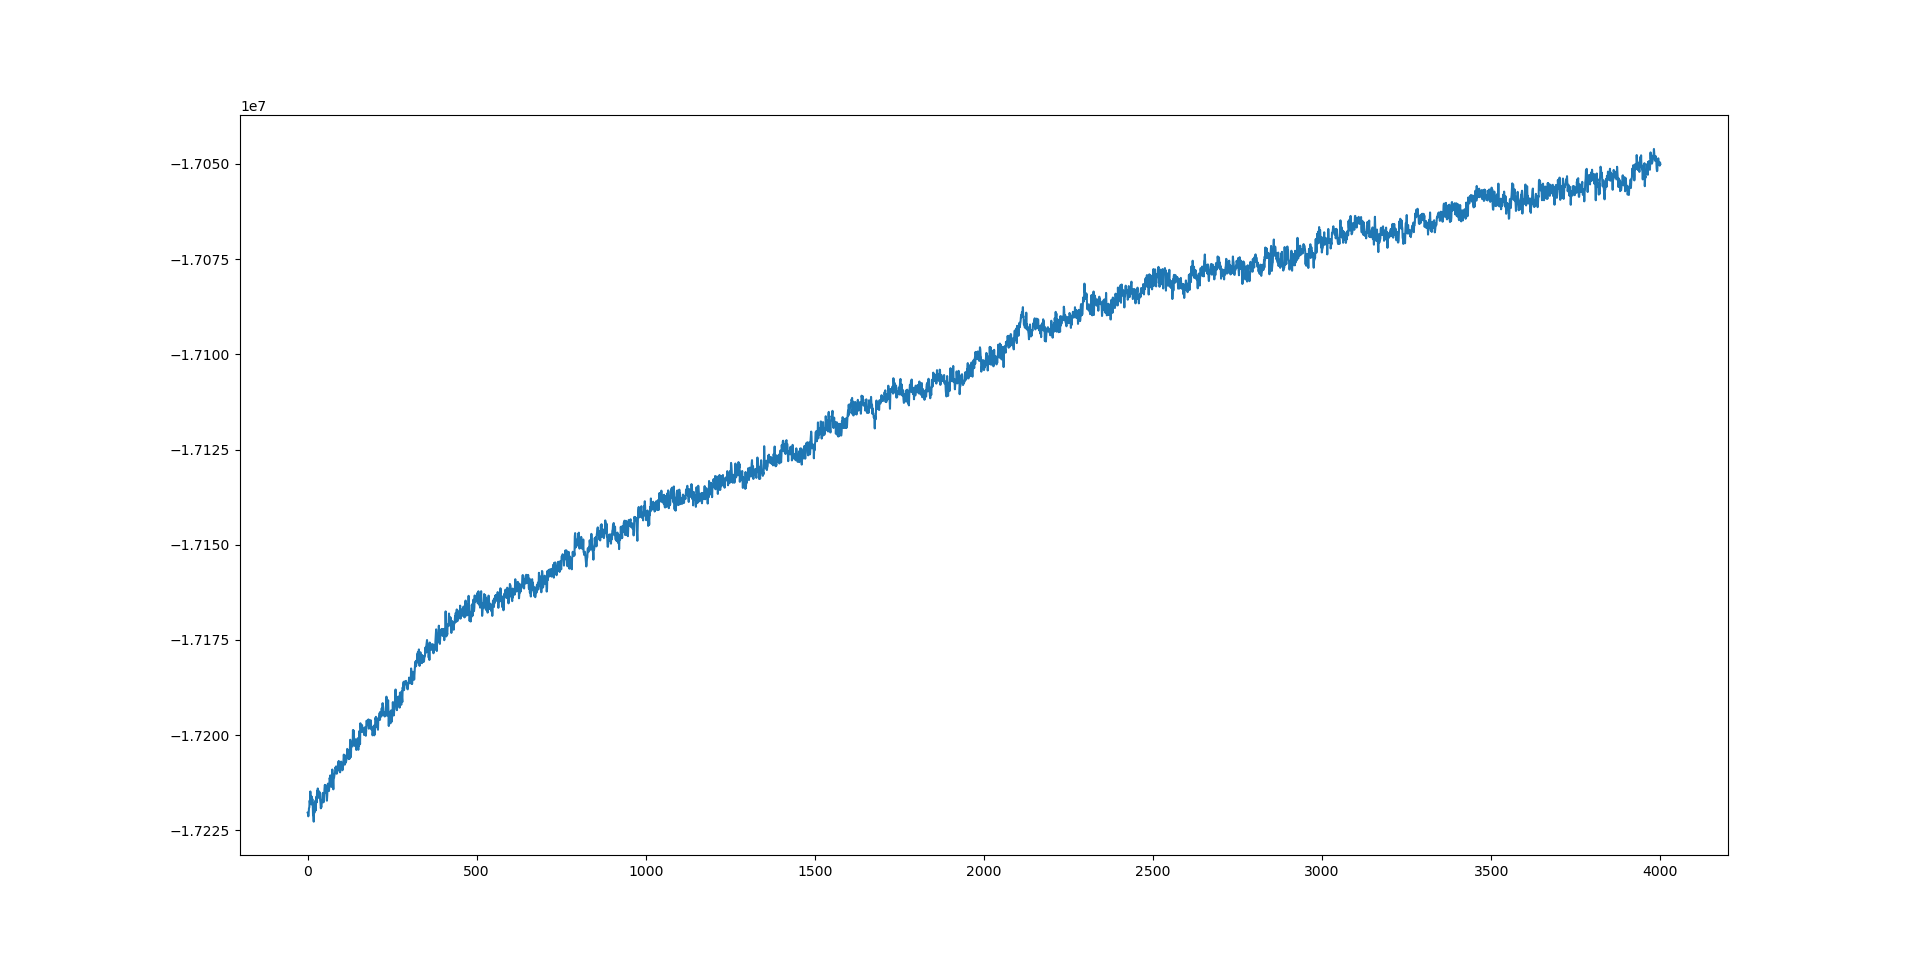
\includegraphics[scale=0.3]{figures/jll_remove_burnin.png}
\end{center}


The 10 most probable words per topic (rows correspond topics)

\begin{flushleft}
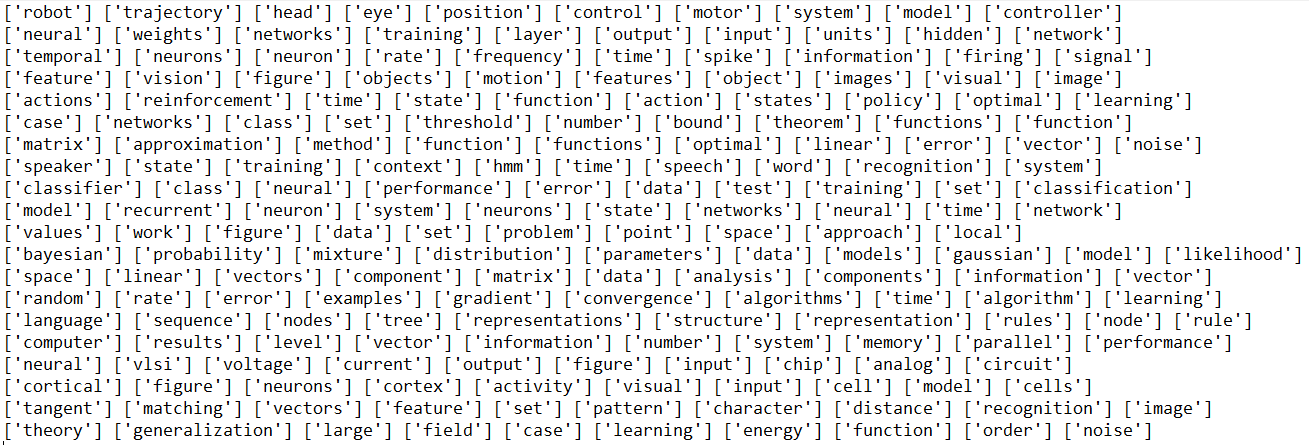
\includegraphics[scale=0.6]{figures/most_probable_words_per_topic.png}
\end{flushleft}



The most similar titles to document 0 are,

\begin{flushleft}
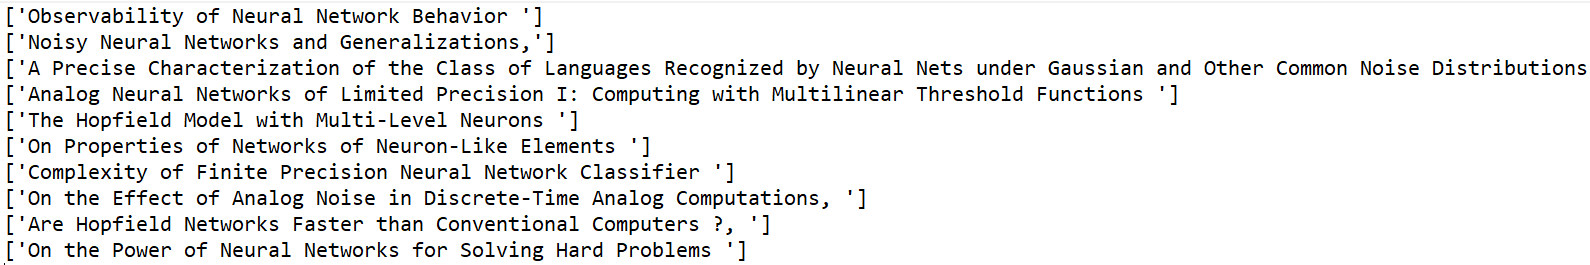
\includegraphics[scale=0.6]{figures/most_similar_titles_to_0}
\end{flushleft}

\newpage

Joint log likelihood code,

\begin{center}
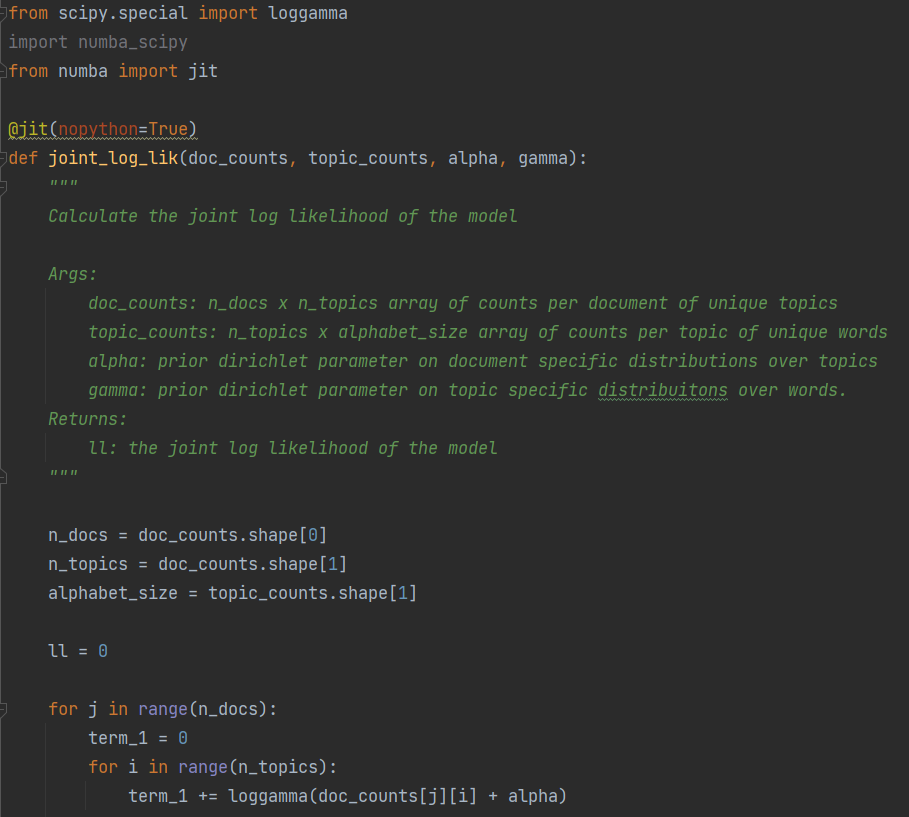
\includegraphics[scale=0.6]{figures/jll_code_1.png}
\end{center}

\begin{center}
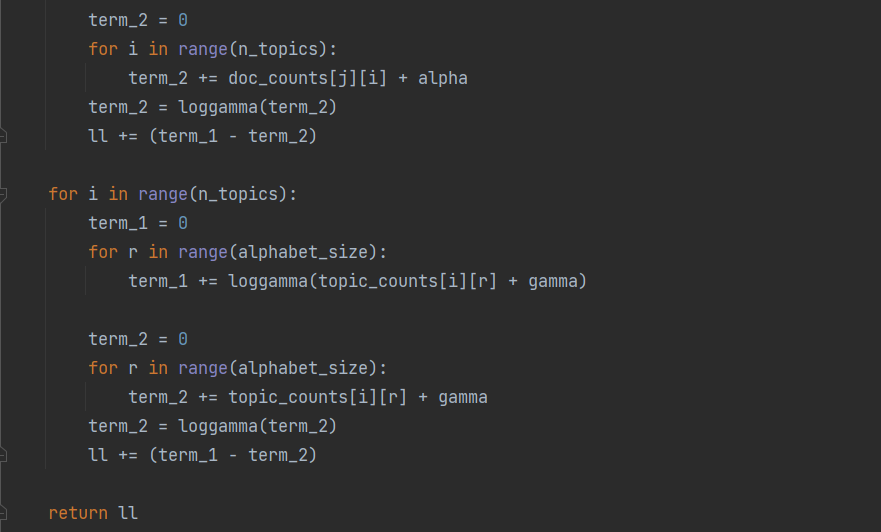
\includegraphics[scale=0.65]{figures/jll_code_2.png}
\end{center}


\newpage

Sampler code,

\begin{center}
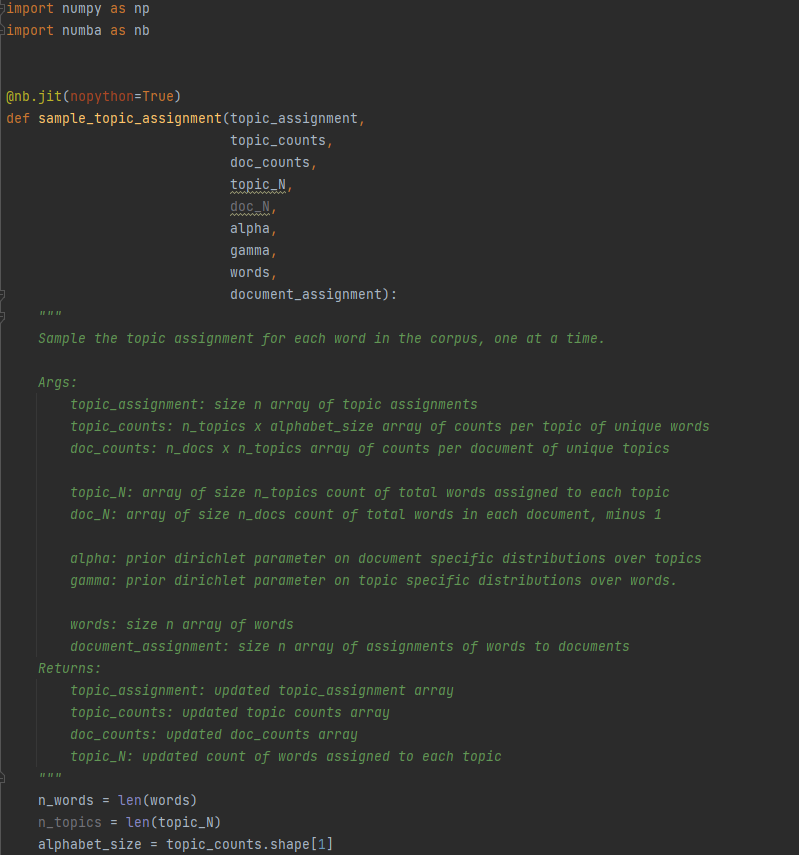
\includegraphics[scale=0.6]{figures/sampler_code_1.png}
\end{center}

\begin{center}
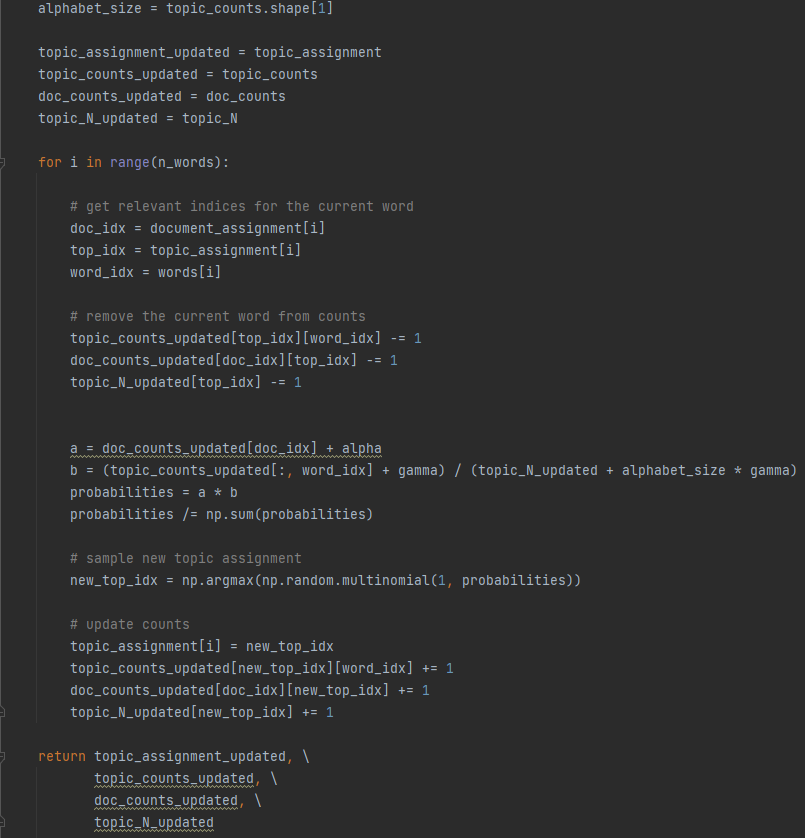
\includegraphics[scale=0.6]{figures/sampler_code_2.png}
\end{center}

\end{document}